\documentclass[conference]{IEEEtran}

% Codificación y lenguaje
\usepackage[utf8]{inputenc} % Codificación de entrada
\usepackage[T1]{fontenc}    % Codificación de fuente
\usepackage[spanish]{babel} % Idioma

% Paquetes útiles
\usepackage{graphicx}
\usepackage{amsmath, amssymb}
\usepackage{cite}
\usepackage{url}
\usepackage[hidelinks]{hyperref}

% Datos del artículo
\title{Especialización de HTNet para reconocimiento multietiqueta de microexpresiones a nivel de unidades de acción}

\author{
  \IEEEauthorblockN{Joel Luis Ibaceta Canchaya}
  \IEEEauthorblockA{
    \textit{Universidad Nacional de Ingeniería} \\
    joel.ibaceta.c@uni.pe
  }
  \and
  \IEEEauthorblockN{Marco Antonio Barrera Ninamango}
  \IEEEauthorblockA{
    \textit{Universidad Nacional de Ingeniería} \\
    marco.barrera.n@uni.pe
  }
  \and
  \IEEEauthorblockN{Jesus Gianpierre Campos Cardenas}
  \IEEEauthorblockA{
    \textit{Universidad Nacional de Ingeniería} \\
    j.campos.c@uni.pe
  }
}

\begin{document}

\maketitle

\begin{abstract}
En este trabajo presentamos una especialización del modelo HTNet para la tarea de reconocimiento multietiqueta de microexpresiones faciales a nivel de unidades de acción (AUs), utilizando el conjunto de datos SAMM V2. A diferencia de aproximaciones tradicionales centradas en la clasificación de emociones compuestas, nuestro enfoque trata cada AU como una etiqueta binaria independiente, permitiendo un análisis más granular y anatómicamente interpretativo.

La arquitectura se ha modificado para producir salidas multietiqueta, aplicando una función de pérdida BCEWithLogitsLoss con pesos ajustados según la frecuencia de cada AU. Además, incorporamos una etapa de normalización facial basada en \textit{Template Matching} antes del cálculo del flujo óptico, mejorando la consistencia espacial entre muestras. Evaluamos el rendimiento del modelo utilizando métricas específicas por AU (F1-score y UAR), demostrando la efectividad del enfoque propuesto para tareas de análisis facial fino, tales como detección de dolor, engaño o emociones compuestas.
\end{abstract}

\begin{IEEEkeywords}
microexpresiones, unidades de acción, HTNet, reconocimiento multietiqueta, visión por computador, SAMM V2
\end{IEEEkeywords}

\section{Introducción}

El reconocimiento automático de expresiones faciales es una disciplina central dentro de la visión por computador, con aplicaciones en interacción humano-máquina, análisis emocional, salud mental, seguridad y estudios de mercado. Tradicionalmente, estos sistemas se han enfocado en predecir emociones discretas como “alegría” o “tristeza”, sin embargo, esta aproximación resulta insuficiente cuando las expresiones son ambiguas, solapadas o sutiles, como ocurre en el caso de las microexpresiones.

Una alternativa más precisa y descomponible es el uso de las \textit{Action Units} (AUs), definidas en el sistema FACS (Facial Action Coding System), desarrollado por Ekman y Friesen. FACS codifica el movimiento facial en términos de contracciones musculares observables, donde cada AU corresponde a un movimiento anatómicamente definido, como el alzamiento interno de las cejas (AU01) o el descenso de la comisura de los labios (AU15). Este enfoque permite analizar expresiones complejas como una combinación de unidades observables, en lugar de etiquetarlas con una única emoción.

Las microexpresiones faciales —movimientos breves e involuntarios que revelan emociones reprimidas— presentan un caso de estudio ideal para el análisis basado en AUs. A diferencia de las expresiones macro, las microexpresiones suelen involucrar la activación de solo algunas AUs por menos de 500 ms, lo que exige modelos sensibles a cambios sutiles y de baja intensidad.

El reconocimiento multietiqueta de AUs —es decir, predecir múltiples AUs activas simultáneamente— habilita aplicaciones de mayor valor añadido. En psicología, permite evaluar reacciones emocionales a nivel muscular, en lugar de simplemente asignar emociones genéricas. En investigación de mercados, facilita la detección de respuestas sutiles no verbalizadas ante productos o mensajes publicitarios. En contextos como entrevistas laborales, permite detectar microexpresiones contradictorias o complementarias, que podrían ser pasadas por alto por clasificadores de emociones tradicionales.

En este trabajo, presentamos una especialización del modelo HTNet, originalmente propuesto para clasificación de microexpresiones, adaptándolo al reconocimiento multietiqueta de AUs en el dataset SAMM V2. Nuestra propuesta incluye modificaciones arquitectónicas orientadas a esta tarea, como una salida por AU y el uso de \texttt{BCEWithLogitsLoss} con ajuste de pesos. Además, incorporamos una etapa de normalización facial mediante \textit{Template Matching}, previa al cálculo del flujo óptico, para mejorar la coherencia espacial entre muestras del dataset. Evaluamos el modelo mediante métricas específicas por AU, como F1-score y UAR, lo que permite validar su capacidad para el análisis detallado de activaciones musculares faciales.

El código fuente, así como los modelos entrenados, están disponibles públicamente en \url{https://github.com/joelibaceta/htnet-microexp-au-multilabel}.

\section{Trabajos Relacionados}

El reconocimiento automático de microexpresiones ha sido abordado mediante diversos enfoques que combinan técnicas de visión por computador y aprendizaje profundo. A continuación, se revisan las líneas principales que fundamentan el presente trabajo, con énfasis en el uso de flujo óptico, la arquitectura HTNet, métodos de alineación facial y el reconocimiento multietiqueta de unidades de acción.

\subsection{Reconocimiento de microexpresiones mediante flujo óptico}

El flujo óptico se ha consolidado como una técnica eficaz para capturar movimientos faciales sutiles entre fotogramas consecutivos. Propuestas como Bi-WOOF \cite{liong2018less} y MDMO \cite{liu2016main} han demostrado que descriptores derivados del flujo óptico permiten distinguir microexpresiones espontáneas con mayor sensibilidad que representaciones basadas en imágenes estáticas. Estas técnicas han sido empleadas tanto en métodos tradicionales como en modelos profundos, debido a su capacidad para preservar la dinámica facial fina.

\subsection{Modelos jerárquicos y HTNet}

La arquitectura HTNet (Hierarchical Transformer Network), propuesta por Chen et al. \cite{chen2023htnet}, introdujo una jerarquía de módulos Transformer para capturar relaciones espaciales y temporales en secuencias de flujo óptico. Su diseño incorpora mecanismos de atención jerárquica y una codificación explícita de la estructura facial. No obstante, el modelo original se orienta a la clasificación de expresiones completas o grupos de AUs, sin una separación explícita por unidad de acción individual.

\subsection{Normalización facial mediante Template Matching}

El preprocesamiento facial mediante técnicas de alineación, como el \textit{Template Matching}, ha sido utilizado para reducir la variabilidad espacial entre muestras antes del análisis expresivo. Aunque su uso ha sido más frecuente en tareas de reconocimiento facial general \cite{pan2011template, liu2015facealignment}, su incorporación en tareas de microexpresión permite mejorar la estabilidad espacial de regiones clave antes del cálculo del flujo óptico. En este trabajo, esta técnica se emplea como una etapa previa al pipeline de reconocimiento.

\subsection{Reconocimiento multietiqueta de unidades de acción}

El reconocimiento multietiqueta de AUs ha sido abordado en contextos de expresión macro, principalmente con datasets como BP4D y DISFA \cite{jaiswal2022deep}. Estos trabajos modelan cada AU como una variable binaria, lo que permite un análisis anatómicamente más interpretativo y reutilizable en dominios clínicos o psicológicos. Sin embargo, este paradigma ha sido menos explorado en tareas de microexpresión, en parte por la escasez de datasets con anotaciones AU frame-a-frame como SAMM V2. 

\section{Metodología}
\subsection{Preprocesamiento de anotaciones del dataset SAMM V2}

El dataset \textit{SAMM V2} (Spontaneous Actions and Micro-Movements) contiene videos de alta resolución con microexpresiones faciales, anotadas manualmente en términos de unidades de acción (AUs) conforme al sistema FACS. Cada muestra incluye un campo de texto llamado \textit{Action Units}, donde las AUs activas se indican mediante notaciones como \texttt{4+7+43A}, que combinan números con sufijos de intensidad.

Para convertir estas anotaciones en vectores multietiqueta, aplicamos una transformación que:
\begin{itemize}
  \item Elimina referencias como \texttt{R}, \texttt{L}, \texttt{A/}, etc.;
  \item Separa las AUs mediante el símbolo \texttt{+};
  \item Convierte cada AU en una columna, y codifica su intensidad en valores continuos entre 0.2 (A) y 1.0 (E), usando un mapa definido por FACS.
\end{itemize}

Este preprocesamiento produce una representación matricial donde cada fila corresponde a una muestra, y cada columna representa una AU con su nivel de activación. A continuación, se muestra un ejemplo de la tabla generada:

\begin{table}[h]
\centering
\begin{tabular}{l|l|c|c|c|c}
\textbf{Archivo} & \textbf{AUs} & AU04 & AU07 & AU43 & AU12 \\
\hline
samm\_001 & 4+7+43A & 1.0 & 1.0 & 0.2 & 0.0 \\
samm\_002 & 6B+12 & 0.4 & 0.0 & 0.0 & 1.0 \\
\end{tabular}
\caption{Ejemplo de transformación del campo \textit{Action Units} a una matriz de intensidades por AU.}
\end{table}

\subsection{Preprocesamiento: Normalización por Template Matching}

Antes de calcular el flujo óptico, es fundamental garantizar que las secuencias de entrada estén alineadas espacialmente. Una mínima variación en la posición o escala del rostro entre cuadros puede introducir artefactos en el flujo resultante, dificultando la detección de cambios sutiles como los que caracterizan a las microexpresiones.

Herramientas ampliamente utilizadas como MTCNN u OpenFace permiten detectar y recortar rostros, pero generan recortes inconsistentes incluso entre cuadros consecutivos visualmente similares.

\begin{figure}[h]
\centering
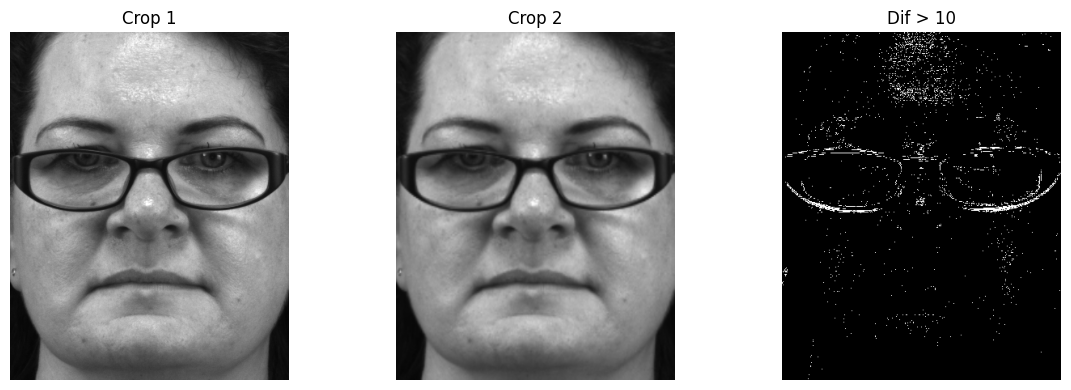
\includegraphics[width=0.9\linewidth]{figs/diff_before.png}
\caption{Diferencias entre recortes consecutivos generados por MTCNN/OpenFace. Incluso entre cuadros visualmente similares se observa desplazamiento.}
\label{fig:before_alignment}
\end{figure}

Para resolver este problema, implementamos una etapa de normalización mediante \textit{Template Matching}, donde se selecciona como plantilla el rostro del primer cuadro de cada secuencia. A través de correlación cruzada 2D, se busca en cada cuadro subsecuente la región que mejor coincide con la plantilla. Esto permite mantener la coherencia espacial entre recortes a lo largo del tiempo.

\begin{figure}[h]
\centering
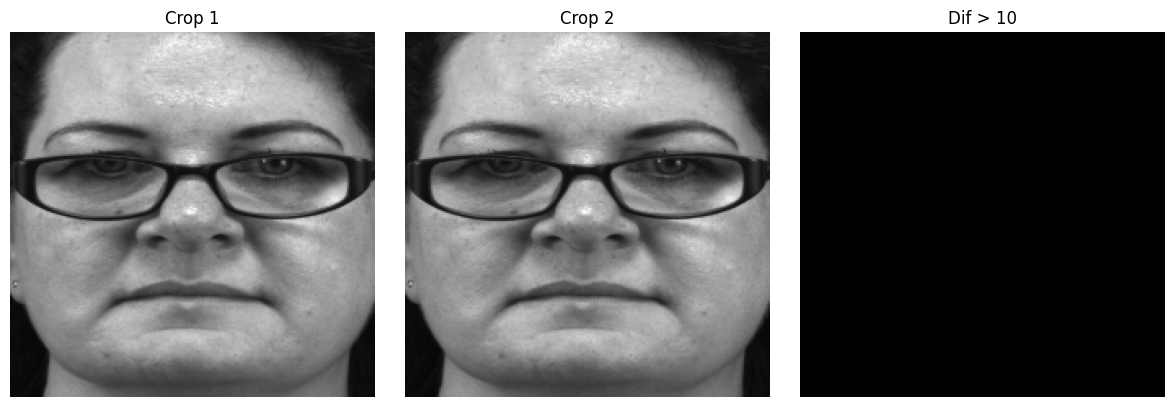
\includegraphics[width=0.9\linewidth]{figs/diff_after.png}
\caption{Diferencia entre cuadros consecutivos luego de aplicar Template Matching. La variación es casi nula, lo que permitirá capturar los movimientos producidos en una microexpresión con mayor precisión.}
\label{fig:after_alignment}
\end{figure}

Adicionalmente, todos los recortes son redimensionados a una resolución fija, lo cual estandariza las entradas al modelo y reduce distorsiones geométricas. Este paso es crucial para preservar la fidelidad del movimiento intercuadro y aumentar la sensibilidad del modelo ante activaciones faciales mínimas.

\subsection{Cálculo del Flujo Óptico}

El flujo óptico es una herramienta central en el análisis de microexpresiones, ya que permite capturar el movimiento sutil de los músculos faciales entre cuadros clave. A diferencia de enfoques que se basan en imágenes estáticas, el flujo óptico proporciona información densa sobre la dinámica del rostro, lo cual es especialmente relevante en el caso de microexpresiones, que ocurren en menos de 500 ms.

Siguiendo trabajos previos como \cite{zhang2023htnet}, el cálculo del flujo óptico se realiza entre los cuadros correspondientes al \textit{onset} (inicio del cambio muscular) y el \textit{apex} (máxima intensidad de la microexpresión), tal como están anotados en el dataset SAMM V2. Este enfoque permite capturar únicamente la variación significativa de la expresión, evitando introducir ruido del contexto neutro.

Utilizamos el método de Farnebäck \cite{farneback2003two}, que estima un campo de movimiento denso mediante aproximaciones cuadráticas de las intensidades locales. Este método es eficiente y se adapta bien a los movimientos pequeños y suaves característicos de las microexpresiones.

Los mapas resultantes de desplazamiento horizontal ($u$) y vertical ($v$) se normalizan y se concatenan como canales de entrada para el modelo, reemplazando las imágenes RGB. Esto permite a la red centrarse exclusivamente en las deformaciones geométricas faciales, reduciendo la influencia de factores como la iluminación o la textura.

\begin{figure}[h]
\centering
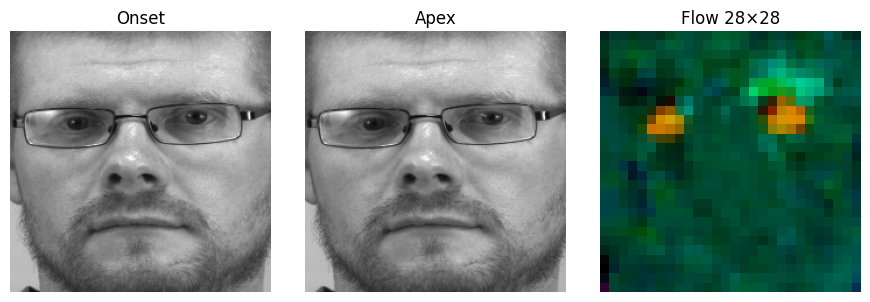
\includegraphics[width=\linewidth]{figs/optical_flow_sample.png}
\caption{Ejemplo del cálculo de flujo óptico entre los cuadros \textit{onset} y \textit{apex} de una microexpresión. A la izquierda se muestra el rostro neutro al inicio de la secuencia; al centro, el cuadro correspondiente al punto de máxima expresión. A la derecha, el mapa de flujo óptico resultante, reducido a una resolución de $28 \times 28$, donde los vectores de movimiento capturan las deformaciones faciales sutiles.}
\label{fig:flow_example}
\end{figure}

\subsection{Adaptación de HTNet a clasificación multietiqueta}

HTNet es una arquitectura jerárquica de atención espacial que combina bloques de transformadores con un esquema de agregación piramidal, permitiendo capturar relaciones espaciales en múltiples escalas. Esta estructura facilita el modelado de dependencias de largo alcance entre regiones dentro de una imagen, manteniendo una resolución progresivamente reducida a través de sus niveles jerárquicos.

Este trabajo parte de la implementación propuesta por Kim et al. (2023)~\cite{kim2023htnet}, quienes aplicaron HTNet al reconocimiento de microexpresiones faciales utilizando mapas de flujo óptico como entrada.

Para adaptarlo al problema de clasificación multietiqueta de Unidades de Acción (AUs), se realizaron las siguientes modificaciones:

\begin{figure}[h]
\centering
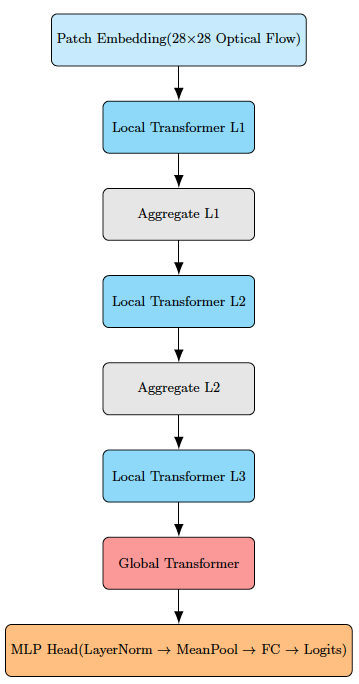
\includegraphics[width=0.6\columnwidth]{figs/custom_htnet_architecture.png}
\caption{Esquema de la arquitectura de HTNet adaptada para clasificación multietiqueta de microexpresiones. La entrada corresponde a mapas de flujo óptico preprocesados (componentes $x$, $y$ y magnitud), embebidos en parches para su procesamiento jerárquico mediante transformadores locales. Cada nivel de atención se combina con operaciones de agregación espacial. Finalmente, se aplica un bloque MLP que reduce la dimensión mediante \texttt{MeanPooling} y proyecta los logits asociados a cada Unidad de Acción (AU). La activación \texttt{sigmoid} no se aplica explícitamente, sino que está implícita en la función de pérdida \texttt{BCEWithLogitsLoss}.}
\label{fig:htnet_diagrama}
\end{figure}


\begin{itemize}
    \item \textbf{Activación de salida:} se reemplazó la función \texttt{softmax} por \texttt{sigmoid}, permitiendo estimar de manera independiente la probabilidad de activación de cada AU.
    
    \item \textbf{Función de pérdida:} se utilizó \texttt{BCEWithLogitsLoss}, que es adecuada para tareas multietiqueta donde una muestra puede pertenecer a varias clases simultáneamente.
    
    \item \textbf{Mantenimiento de la entrada:} dado que la implementación original ya procesaba mapas de flujo óptico con tres canales (componentes $x$, $y$ y magnitud), no fue necesario modificar la primera capa del modelo.
\end{itemize}

\begin{table}[h]
\centering
\resizebox{\columnwidth}{!}{%
\begin{tabular}{|l|c|c|}
\hline
\textbf{Característica} & \textbf{HTNet} & \textbf{Versión Adaptada} \\
\hline
Tipo de entrada & Flujo óptico & Flujo óptico Normalizado \\
\hline
Dimensión de entrada & 3 canales & 3 canales \\
\hline
Tarea & Clasificación Multicategoria & Clasificación multietiqueta \\
\hline
Salida & Logits (una clase) & Logits (múltiples AUs) \\
\hline
Función de pérdida & Cross Entropy & BCEWithLogitsLoss \\
\hline
Normalización & LayerNorm por canal & Igual (sin cambios) \\
\hline
\end{tabular}
}
\caption{Comparación entre HTNet de Kim et al. (2023) y la versión adaptada para clasificación multietiqueta de unidades de acción.}
\label{tab:htnet_vs_adaptado}
\end{table}



\subsection{Función de pérdida y métricas utilizadas}

Dado que la tarea de detección de unidades de acción facial (AUs) se plantea como un problema de clasificación multietiqueta, se utilizó la función de pérdida \texttt{BCEWithLogitsLoss} provista por PyTorch. Esta función combina de forma eficiente una sigmoide sobre las salidas del modelo con la pérdida de entropía cruzada binaria, evitando problemas numéricos y mejorando la estabilidad durante el entrenamiento.

Para abordar el marcado desbalance en la frecuencia de aparición de las AUs, se calculó un vector de pesos positivos (\texttt{pos\_weight}) proporcional a la inversa de la frecuencia relativa de cada clase. Esto permite penalizar más fuertemente los errores en clases minoritarias, incentivando una mejor detección de AUs infrecuentes.

Durante la validación, las salidas del modelo fueron transformadas en probabilidades aplicando la función sigmoide. Posteriormente, se aplicó un umbral fijo ($\tau = 0{,}5$) para binarizar las predicciones y calcular métricas de desempeño. Las métricas empleadas fueron \textbf{precisión}, \textbf{recobrado (recall)} y \textbf{F1-score}, todas con promedio \textit{macro}, lo cual asegura que cada AU tenga igual peso en la evaluación, independientemente de su prevalencia. Estas métricas permiten evaluar de forma robusta el rendimiento del modelo en contextos multietiqueta con clases desbalanceadas.



\section{Experimentos}


\subsection{Entrenamiento y configuración experimental}

El entrenamiento del modelo se realizó utilizando el conjunto de datos SAMM, procesado previamente en forma de mapas de flujo óptico entre pares de fotogramas. Las imágenes fueron transformadas únicamente mediante la conversión a tensores utilizando \texttt{ToTensor()}.

Se empleó el optimizador \texttt{Adam} con una tasa de aprendizaje de $1 \times 10^{-4}$ y un tamaño de lote (\textit{batch size}) de 16. El proceso de entrenamiento se ejecutó durante un máximo de 10 épocas, con la estrategia de \textit{early stopping} activada si no se observaba mejora en la pérdida de validación después de una época.

La función de pérdida utilizada fue \texttt{BCEWithLogitsLoss}, adecuada para el caso de clasificación multietiqueta. Se calculó un vector de pesos \texttt{pos\_weight} a partir de la frecuencia relativa de aparición de cada acción facial (AU) para abordar el desbalance de clases, aunque este no fue finalmente incorporado en la función de pérdida.

El conjunto de datos se dividió en entrenamiento y validación utilizando \texttt{GroupShuffleSplit}, garantizando que los sujetos no se repitan entre ambos subconjuntos. Esto reduce el sesgo por identidad en la evaluación. El seguimiento y registro del entrenamiento, incluyendo pérdidas, distribuciones de activación y ejemplos de predicción, fue gestionado mediante la herramienta \texttt{Weights \& Biases (wandb)}.

Durante el proceso de entrenamiento, se observó una reducción progresiva tanto de la pérdida en el conjunto de entrenamiento como en el de validación, como se muestra en la Figura~\ref{fig:loss_curves}, lo que sugiere una convergencia adecuada del modelo sin indicios evidentes de sobreajuste.

\begin{figure}[ht]
    \centering
    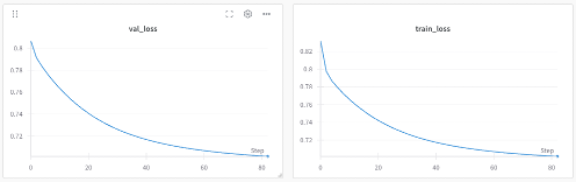
\includegraphics[width=\columnwidth]{figs/metrics.png}
    \caption{Arriba: curvas de pérdida para entrenamiento y validación a lo largo de 50 épocas. Abajo: matrices de confusión para las unidades de acción AU\_04, AU\_07 y AU\_21.}
    \label{fig:loss_curves}
\end{figure}
\begin{figure}[ht]
    \centering
    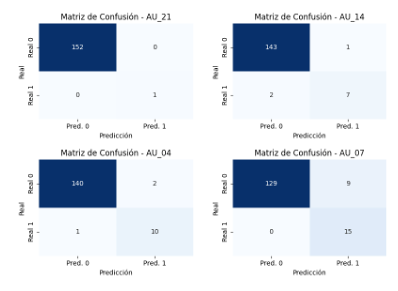
\includegraphics[width=\columnwidth]{figs/AUS_GRID.png}
    \label{fig:loss_curves}
\end{figure}

Se analizaron matrices de confusión para distintas unidades de acción con el fin de evaluar el desempeño individual del modelo. En la \textbf{AU\_04}, el modelo detectó correctamente 10 de los 11 casos positivos, mostrando sensibilidad adecuada y pocos falsos positivos. La \textbf{AU\_07} también presentó buenos resultados con 15 verdaderos positivos, aunque acompañados de algunos falsos positivos. En contraste, las AUs \textbf{AU\_14} y \textbf{AU\_21}, al estar poco representadas, mostraron alta especificidad pero menor sensibilidad, indicando un posible sesgo hacia la clase negativa.


\subsection{Resultados cualitativos}

Para evaluar la capacidad generalizadora del modelo más allá del conjunto de entrenamiento, se realizaron predicciones sobre videos externos que no pertenecen al conjunto de datos utilizado durante la etapa de entrenamiento o validación. Estos videos muestran expresiones faciales espontáneas y fueron procesados mediante nuestro sistema para identificar automáticamente las Unidades de Acción (AUs) activadas.


\begin{figure}[h]
    \centering
    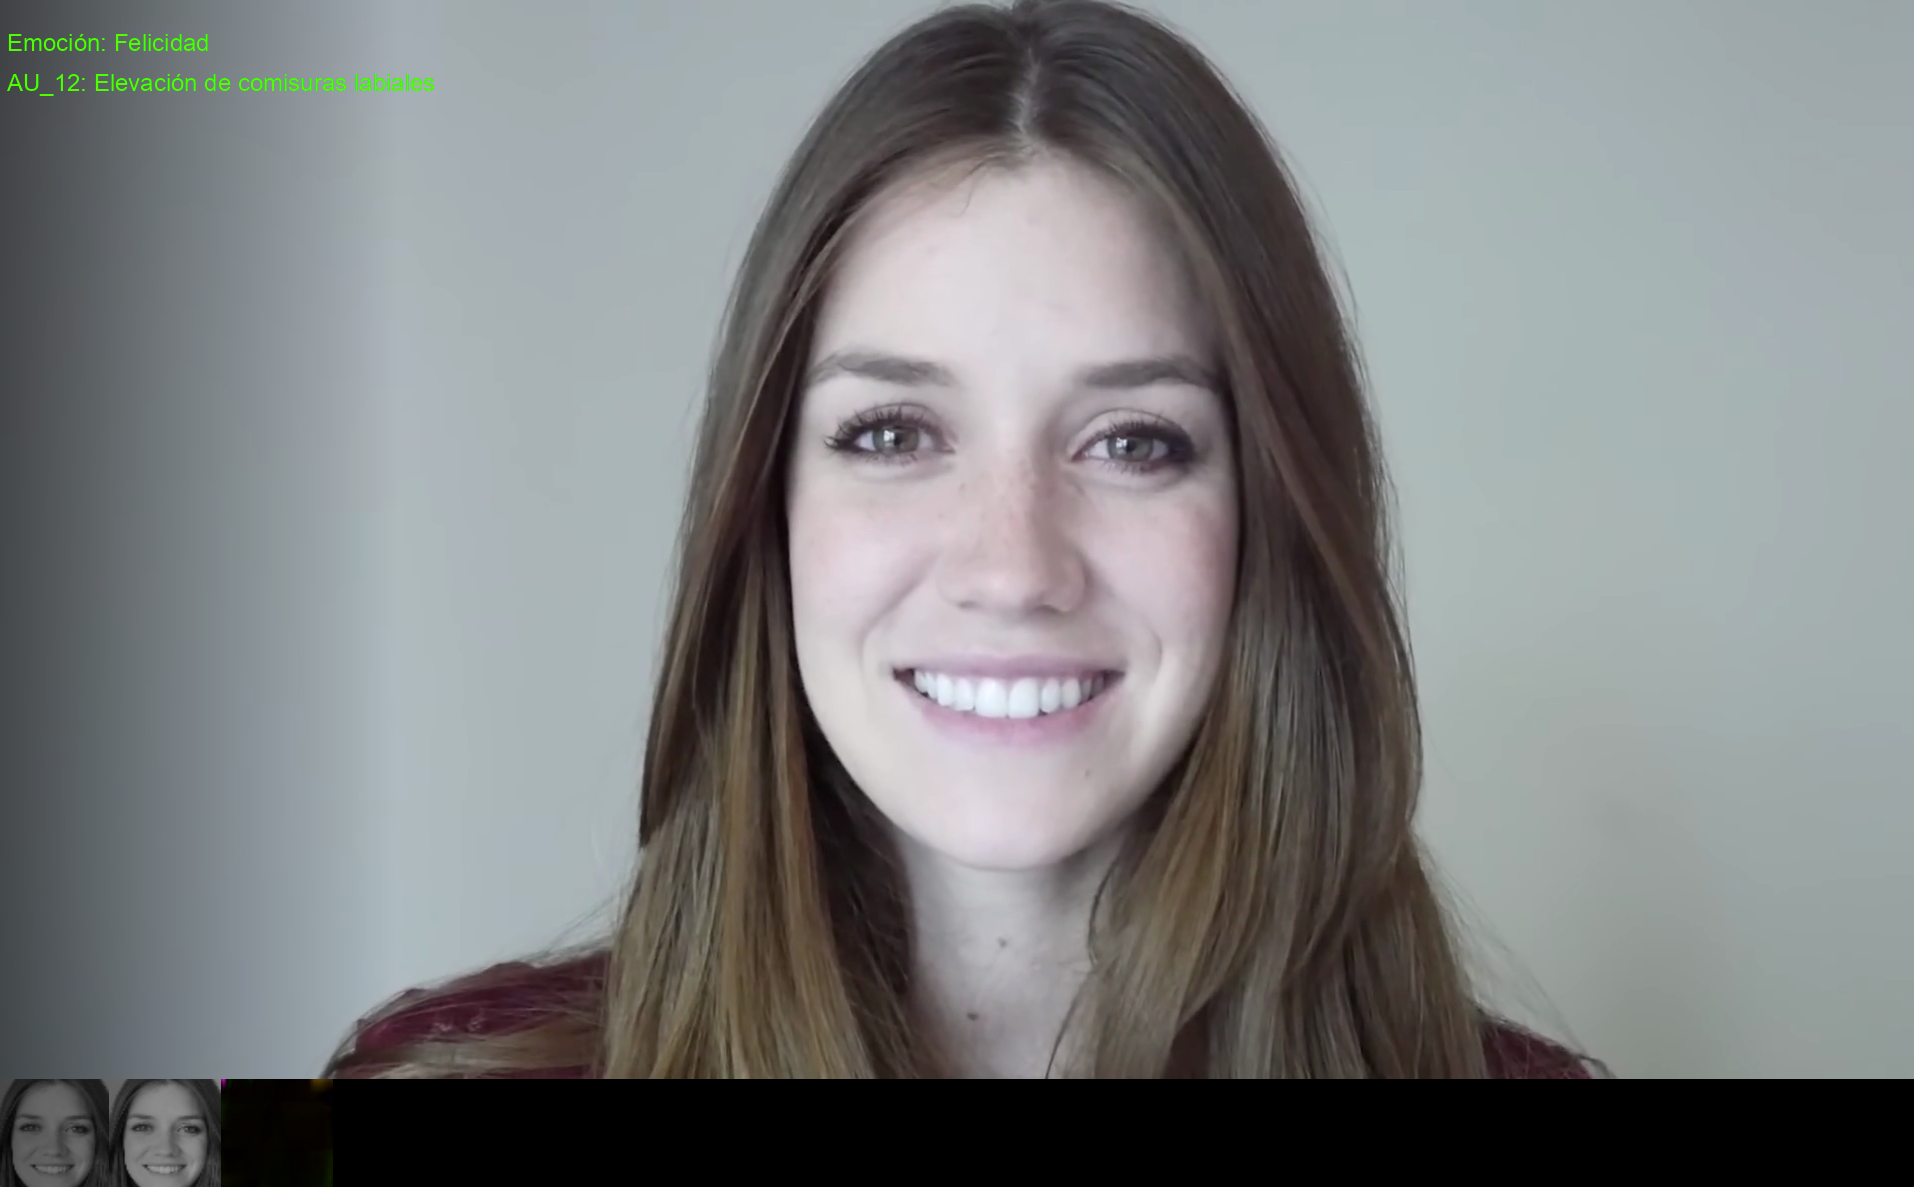
\includegraphics[width=0.45\textwidth]{figs/qualitative_happy.png}
    \caption{Detección de AUs relacionadas con la emoción de felicidad en un video externo. El modelo identifica correctamente la AU\_12, típica de la sonrisa.}
    \label{fig:qualitative_happy}
\end{figure}

\begin{figure}[h]
    \centering
    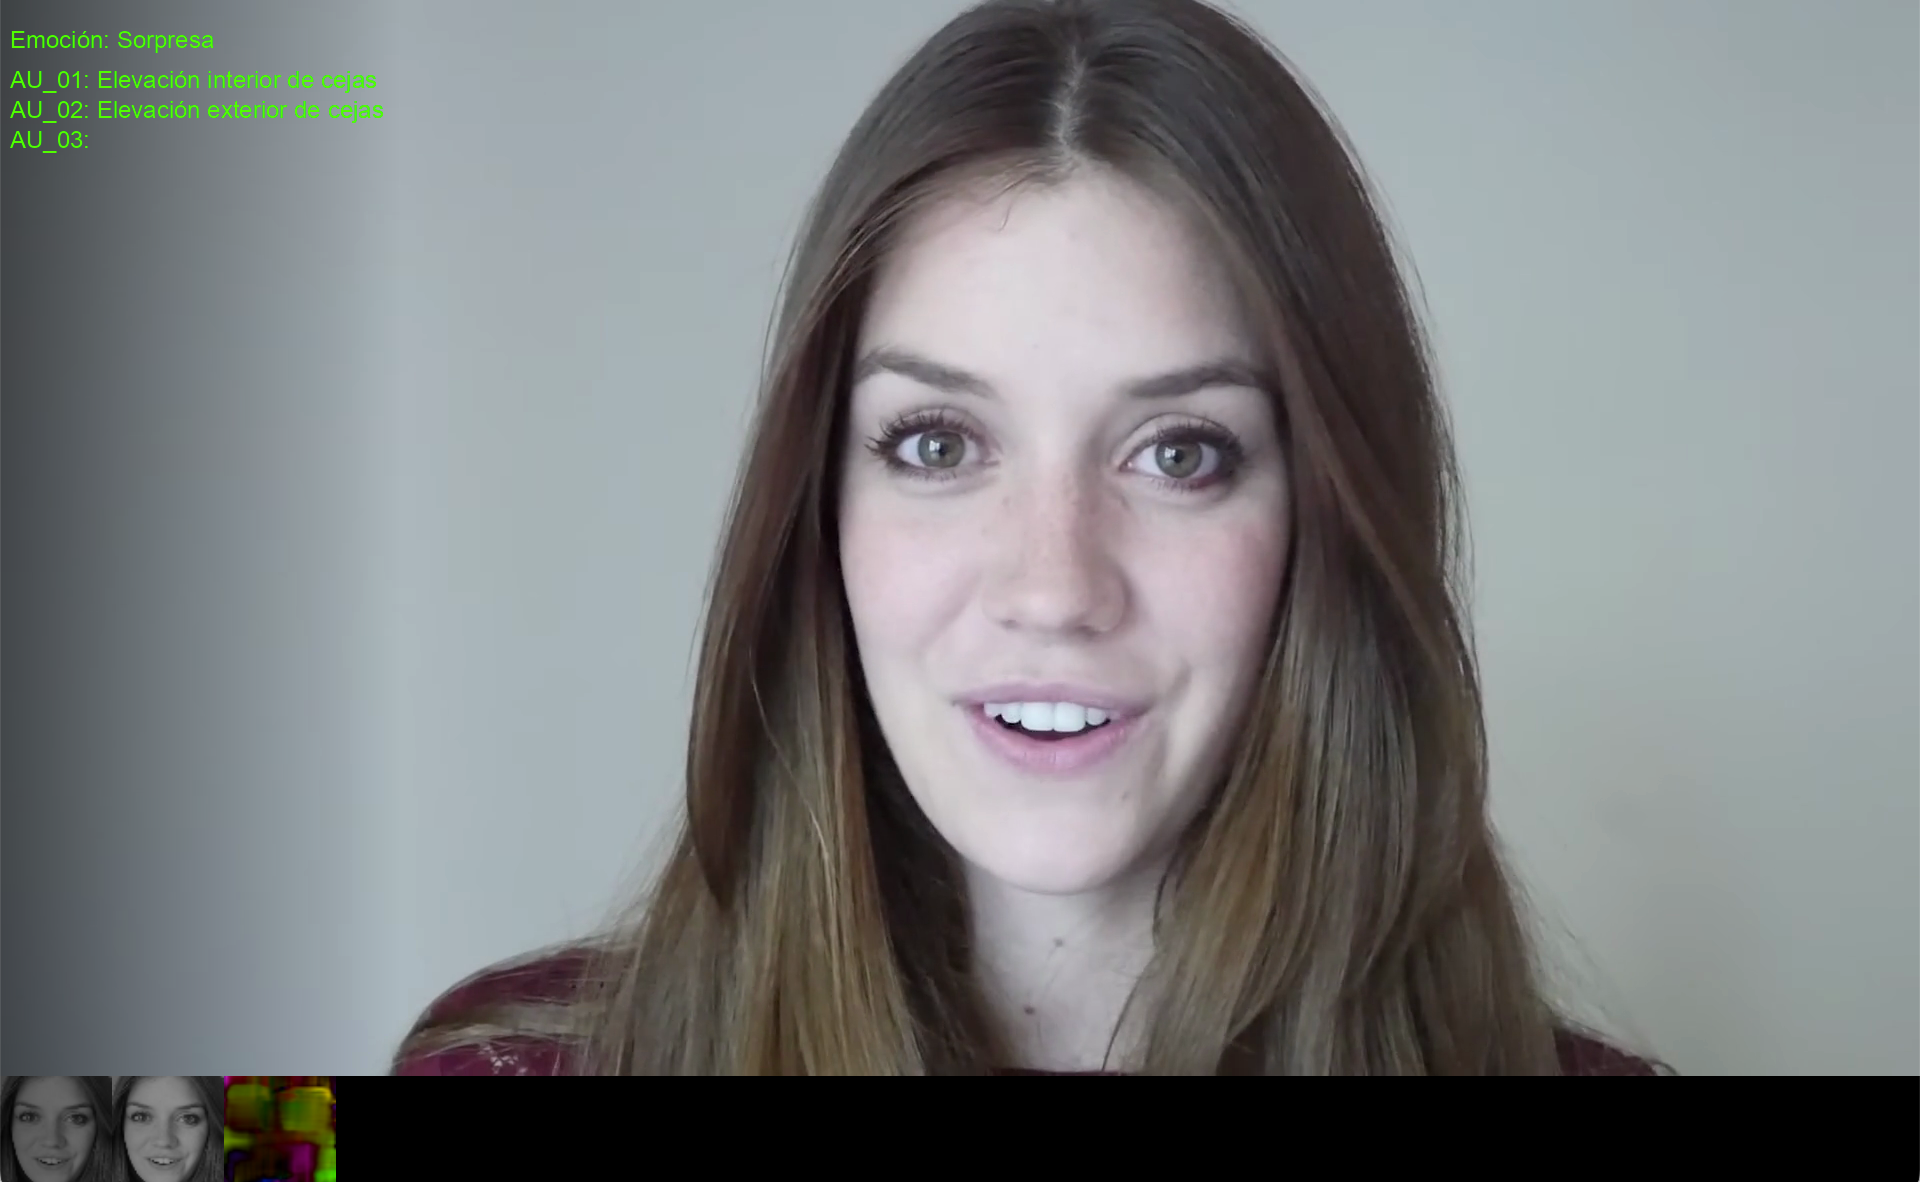
\includegraphics[width=0.45\textwidth]{figs/qualitative_surprise.png}
    \caption{Detección de AUs relacionadas con la emoción de sorpresa. Se activan AU\_01, AU\_02 y AU\_03, vinculadas con el levantamiento de cejas.}
    \label{fig:qualitative_surprise}
\end{figure}

En las Figuras~\ref{fig:qualitative_happy} y~\ref{fig:qualitative_surprise} se observan ejemplos de detecciones exitosas realizadas por el modelo. En particular, se aprecia la activación coherente de la \texttt{AU\_12} (elevación de comisuras labiales), típicamente asociada con la emoción de felicidad, así como de las \texttt{AU\_01}, \texttt{AU\_02} y \texttt{AU\_03}, que corresponden a patrones musculares vinculados con la sorpresa.

Estas salidas ilustran un caso de uso práctico donde el modelo puede integrarse como base para un sistema de reconocimiento emocional utilizando las reglas del sistema FACS (Facial Action Coding System), permitiendo una inferencia interpretativa de las emociones humanas a partir de expresiones microfaciales.


\section{Conclusiones}

En este trabajo se implementó un modelo de clasificación multietiqueta basado en HTNet para la detección de unidades de acción facial (AUs) en secuencias de microexpresiones utilizando flujos ópticos. El modelo mostró capacidad para aprender patrones temporales relevantes incluso en un conjunto de datos limitado y con alta desbalance de clases, logrando una inferencia en tiempo real con un promedio de 1.92 ms por frame.

La incorporación de \textit{template matching} y flujo óptico HSV permitió replicar condiciones similares a las del dataset en videos externos, y validar así la generalización del modelo en entornos no controlados. Esto sugiere un potencial uso del modelo en aplicaciones interactivas y de análisis emocional, como sistemas de retroalimentación en tiempo real o herramientas de investigación psicológica.

Además, se demostró que la arquitectura es lo suficientemente ligera y robusta como para ser integrada en una aplicación web, lo cual amplía su portabilidad y usabilidad en contextos académicos o clínicos.

Como trabajo futuro se plantea ampliar el conjunto de datos, refinar las etiquetas de AUs mediante validación por expertos, y explorar arquitecturas más especializadas para modelar mejor las relaciones espaciales y temporales entre unidades de acción.


\section*{Contribuciones de los autores}

\textbf{Joel Luis Ibaceta Canchaya} lideró el desarrollo del modelo de clasificación multietiqueta basado en HTNet, incluyendo el diseño de los experimentos, la adaptación del flujo de entrenamiento y la configuración de la función de pérdida y métricas. Además, se encargó del preprocesamiento de datos, del análisis de resultados y de la integración con herramientas de seguimiento como \texttt{Weights \& Biases}.

\textbf{Marco Antonio Barrera Ninamango} estuvo a cargo de la construcción de la interfaz de usuario, la captura en tiempo real, la visualización de resultados y la integración del modelo en una aplicación funcional. También colaboró en la evaluación cualitativa utilizando videos externos y en la generación de material gráfico.

\textbf{Jesus Gianpierre Campos Cardenas} contribuyó con la revisión bibliográfica, la organización y redacción del artículo, el formateo en \LaTeX{}, y la edición final del documento. Además, construyó una versión web de la aplicación, demostrando la portabilidad del modelo a contextos ligeros y multiplataforma. 



\begin{thebibliography}{9}

\bibitem{liong2018less}
Liong, S.T., See, J., Wong, K., \& Phan, R. C.W. (2018).
Less is More: Micro-expression Recognition from Video using Apex Frame.
\textit{IEEE Transactions on Affective Computing}.

\bibitem{liu2016main}
Liu, Y.J., Zhang, J.K., Yan, W.J., Wang, S.J., Zhao, G., \& Fu, X. (2016).
A Main Directional Mean Optical Flow Feature for Spontaneous Micro-Expression Recognition.
\textit{IEEE Transactions on Affective Computing}.

\bibitem{li2019ofbp}
Li, X., Hong, X., Moilanen, A., Huang, X., Pfister, T., Zhao, G., \& Pietikäinen, M. (2019).
Towards Reading Hidden Emotions: A Comparative Study of Spontaneous Micro-expression Spotting and Recognition Methods.
\textit{IEEE Transactions on Affective Computing}.

\bibitem{chen2023htnet}
Chen, T., Wang, D., Ji, X., \& Chen, L. (2023).
HTNet: Hierarchical Transformer Networks for Micro-Expression Recognition.
\textit{arXiv preprint arXiv:2307.14637}.

\bibitem{pan2011template}
Pan, W., et al. (2011).
Template Matching-Based Eye Detection in Facial Images.
\textit{International Conference on Advanced Computer Control}.

\bibitem{liu2015face}
Liu, Y. \& Zhang, J. (2015).
Face alignment by explicit shape regression.
\textit{International Journal of Computer Vision}.

\bibitem{jaiswal2022deep}
Jaiswal, A., Valstar, M., \& Almaev, T. (2022).
Deep Multi-label AU Recognition for Expression Analysis.
\textit{Computer Vision and Image Understanding}.

\bibitem{kim2023htnet}
Y. Kim, Y. Cho, S. Yoon, J. Kim, and J. Park, ``HTNet: Hierarchical Transformer for Facial Expression Recognition,'' \textit{arXiv preprint arXiv:2307.14637}, 2023.

\bibitem{joelibaceta2025samm}
Joel Luis Ibaceta Canchaya.
\newblock \emph{SAMM Optical Flow Preprocessing - 28x28 crops}.
\newblock GitHub repository. Available at: \url{https://github.com/joelibaceta/samm-optflow-28}, Accessed: June 14, 2025.

\bibitem{joelibaceta2025htnet}
Joel Luis Ibaceta Canchaya.
\newblock \emph{HTNet for Micro-expression AU Multi-label Classification}.
\newblock GitHub repository. Available at: \url{https://github.com/joelibaceta/htnet-microexp-au-multilabel}, Accessed: June 14, 2025.

\bibitem{samm} D. Davison, M. Lansley, N. Costen, C. Tan, M. Yap. "SAMM: A Spontaneous Micro-Facial Movement Dataset." IEEE Transactions on Affective Computing, 2016.

\bibitem{wandb} Biewald, L. (2020). Experiment tracking with Weights and Biases. Software available from wandb.com.

\end{thebibliography}

\end{document}